
\definecolor{tableheader}{rgb}{0.8, 0.8, 0.8}
\definecolor{tableevenrow}{rgb}{0.95, 0.95, 0.95}
\definecolor{tableoddrow}{rgb}{1.0, 1.0, 1.0}

%----------------------------------------------------------------------------------------
\chapter{Contesto lavorativo}
\label{cap:introduzione}
\section{Profilo aziendale}
Zero12 s.r.l. è una \textit{startup} italiana fondata nel 2012, con attualmente due sedi operative: una a Padova (dove ho svolto il periodo di \textit{stage}) e una ad Empoli. 
L'azienda è \textit{partner} \gls{awsg}, una piattaforma di servizi \textit{cloud} offerta da Amazon, ed è specializzata nella realizzazione di applicazioni \textit{cloud native} e dello sviluppo di applicazioni e servizi \textit{web} e \textit{mobile}, offrendo ai propri clienti, proveniente da ambiti diversificati, soluzioni flessibili e scalibili.\\
Il team di Zero12 s.r.l. non si limita alla realizzazione di applicazioni, ma si estende alla creazione di un percorso di innovazione condiviso con i clienti. Questo percorso mira a integrare nelle realtà aziendali le tecnologie più adatte alle specifiche esigenze, assicurando un miglioramento continuo dei processi aziendali e un’efficace presenza sul web.\\
L'azienda è parte di Var Group s.p.a, un' azienda italiana che fornisce ai propri \textit{partner}, servizi e competenze per raggiungere gli obiettivi prefissati.
\section{Organizzazione aziendale}
Durante il mio periodo di \textit{stage} ho avuto modo osservare in prima persona l'organizzazione in \textit{team} di lavoro che l'azienda adotta.
I ruoli che ho potuto osservare sono rappresentati di seguito nella tabella \ref{tab:ruoli}.
\begin{longtable}{|>{\RaggedRight\arraybackslash}p{3.5cm}|>{\RaggedRight\arraybackslash}p{8.5cm}|}
    \hline
    \rowcolor{tableheader}\textbf{Ruolo} & \textbf{Descrizione} \\
    \hline
    \endfirsthead

    \rowcolor{tableheader}\textbf{Ruolo} & \textbf{Descrizione} \\
    \hline
    \endhead

    \hline
    \endfoot

    \hline
    \endlastfoot
    \hline
    \rowcolor{tableoddrow}\textbf{\textit{CEO}} & Il \gls{ceog} rappresenta il ruolo più alto all'interno dell'azienda. È responsabile nel definire la strategia e le decisioni più importanti dell'azienda. Supervisiona i processi aziendali e gestisce i contatti con potenziali nuovi clienti. \\
    \hline
    \rowcolor{tableevenrow}\textbf{\textit{Project manager}} & Il \textit{project manager} è la figura che si occupa di coordinare il proprio team di lavoro, gestendo le risorse e le tempistiche di progetto e interfacciandosi con il cliente.\\
    \hline
    \rowcolor{tableoddrow}\textbf{\textit{Software developer}} & Il \textit{software developer} è la figura che si occupa della progettazione e dello sviluppo delle varie componenti \textit{software} individuate durante la fase di analisi e progettazione. Ognuno di loro si specializza nello sviluppo di funzionalità di \textit{frontend}, \textit{backend} o entrambi (\textit{fullstack}) a seconda delle competenze e delle preferenze personali.\\
    \hline
    \rowcolor{tableevenrow}\textbf{\textit{Mobile developer}} & Il \textit{mobile developer} è la figura che si occupa della stessa mansione del \textit{software developer}, per un'applicazione \textit{mobile}. All'interno dell'azienda Zero12 s.r.l. i \textit{mobile developers} si suddividono in due categorie: \textit{Android developers} e \textit{iOS developers}.\\
    \hline
    \rowcolor{tableoddrow}\textbf{\textit{AWS specialist}} & L'\textit{AWS Specialist} è la figura specializzata nella configurazione, gestione e adozione dei servizi offerti da \gls{aws}.\\
    \hline
    \rowcolor{tableevenrow}\textbf{\textit{HR}} & La figura dell' \gls{hrg} è una figura che si occupa della gestione delle risorse umane all'interno dell'azienda.\\
    \hline
    \caption{Organizzazione dei ruoli all'interno di Zero12 s.r.l.}
    \label{tab:ruoli}
\end{longtable}

\noindent
Ad ogni nuovo progetto viene assegnato un \textit{team} di lavoro composto da un \textit{project manager}, un numero variabile di \textit{software developers} o \textit{mobile developers}, a seconda delle esigenze del progetto, e un \textit{AWS specialist} se il progetto prevede l'utilizzo di servizi \gls{aws}. 
\pagebreak
\section{Processi aziendali}
\subsection{Metodologia di sviluppo}
Durante il mio periodo di \textit{stage} ho avuto modo di sperimentare in prima persona i processi istanziati dall'azienda per la realizzazione di un progetto.
La metodologia di lavoro adottata è quella \textit{Agile} e in particolare il \textit{framework Scrum}.\\ 
Il \textit{framework Scrum} prevede la suddivisione del progetto in \textit{Sprint} di durata fissa (durante il mio periodo di \textit{stage} la durata era di una settimana) e la definizione di un \textit{team} di lavoro (il \textit{team} di lavoro era composto dal mio \textit{tutor} aziendale come \textit{project manager} e da me come \textit{software developer}).
\begin{figure}[H]
    \centering
    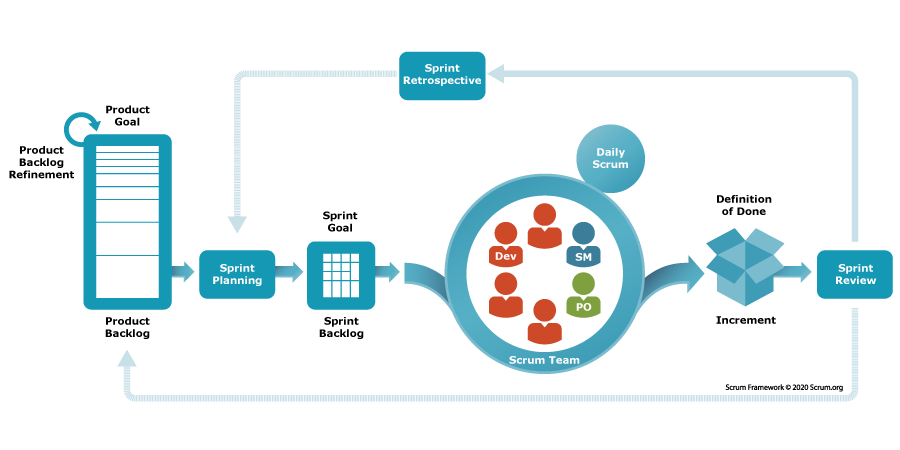
\includegraphics[width=0.9\textwidth]{scrum.png}
    \caption{Schema di flusso di un progetto con metodologia \textit{Scrum}}
    \small \textbf{Fonte:} \url{scrum.org}
    \label{fig:scrum}
\end{figure}
\noindent
Nella figura \ref{fig:scrum} viene mostrato il flusso di lavoro di un progetto con metodologia \textit{Scrum}. All'interno dell'azienda, il flusso di lavoro segue il seguente schema:
\begin{itemize}
    \item \textit{\gls{User-stories}}: all'inizio viene effettuata una prima sessione di \textit{user stories mapping} che va a definire quello che sarà presente nel \textit{product backlog}. Questa sessione viene svolta insieme al cliente, in modo da avere una chiara visione delle aspettative del cliente, definendo cosi anche le \textit{feature} più importanti da sviluppare.
    \item \textbf{\textit{Sprint planning}}: all'inizio di ogni \textit{sprint} vengono selezionate le \textit{task} da svolgere, in base alla priorità, dal \textit{product backlog} e vengono assegnate ai membri del \textit{team} di lavoro.
    \item \textbf{\textit{Sprint review}}: alla fine di ogni \textit{sprint} viene effettuata una revisione del lavoro svolto, andando a controllare che le \textit{task} assegnate siano completate e che il lavoro assegnato, sia stato svolto in modo conforme alle aspettative del cliente.
    \item \textbf{\textit{Sprint retrospective}}: alla fine di ogni \textit{sprint} viene effettuato un controllo interno del lavoro svolto durante lo \textit{sprint}, andando ad evidenziare eventuali problematiche sorte e andando a definire eventuali miglioramenti da apportare al processo di lavoro.
\end{itemize}
\subsection{Strumenti di supporto ai processi}
\subsubsection{Jira}
\textit{Jira} è un \gls{itsg} sviluppato da \textit{Atlassian} che permette la gestione dei progetti in modo \textit{Agile}. Inoltre permette la gestione di \textit{ticket} e la creazione di \textit{board} personalizzate per la gestione dei progetti.
All'inizio di ogni \textit{sprint}, lo \textit{scrum master} crea una nuova \textit{board} relativa allo \textit{sprint} in corso e assegna le \textit{task} da svolgere ai membri del \textit{team} di lavoro.
I membri del \textit{team} di lavoro posso spostare i \textit{ticket} da una colonna all'altra: 
\begin{itemize}
    \item \textbf{Da completare}: \textit{Ticket} assegnati ma che devono essere ancora completati.
    \item \textbf{In corso}: \textit{Ticket} assegnati ad una o più risorse del \textit{team} di lavoro e che sono in fase di sviluppo.
    \item \textbf{Completato}; \textit{Ticket} completati e pronti per la revisione.
\end{itemize}
\begin{figure}[H]
    \centering
    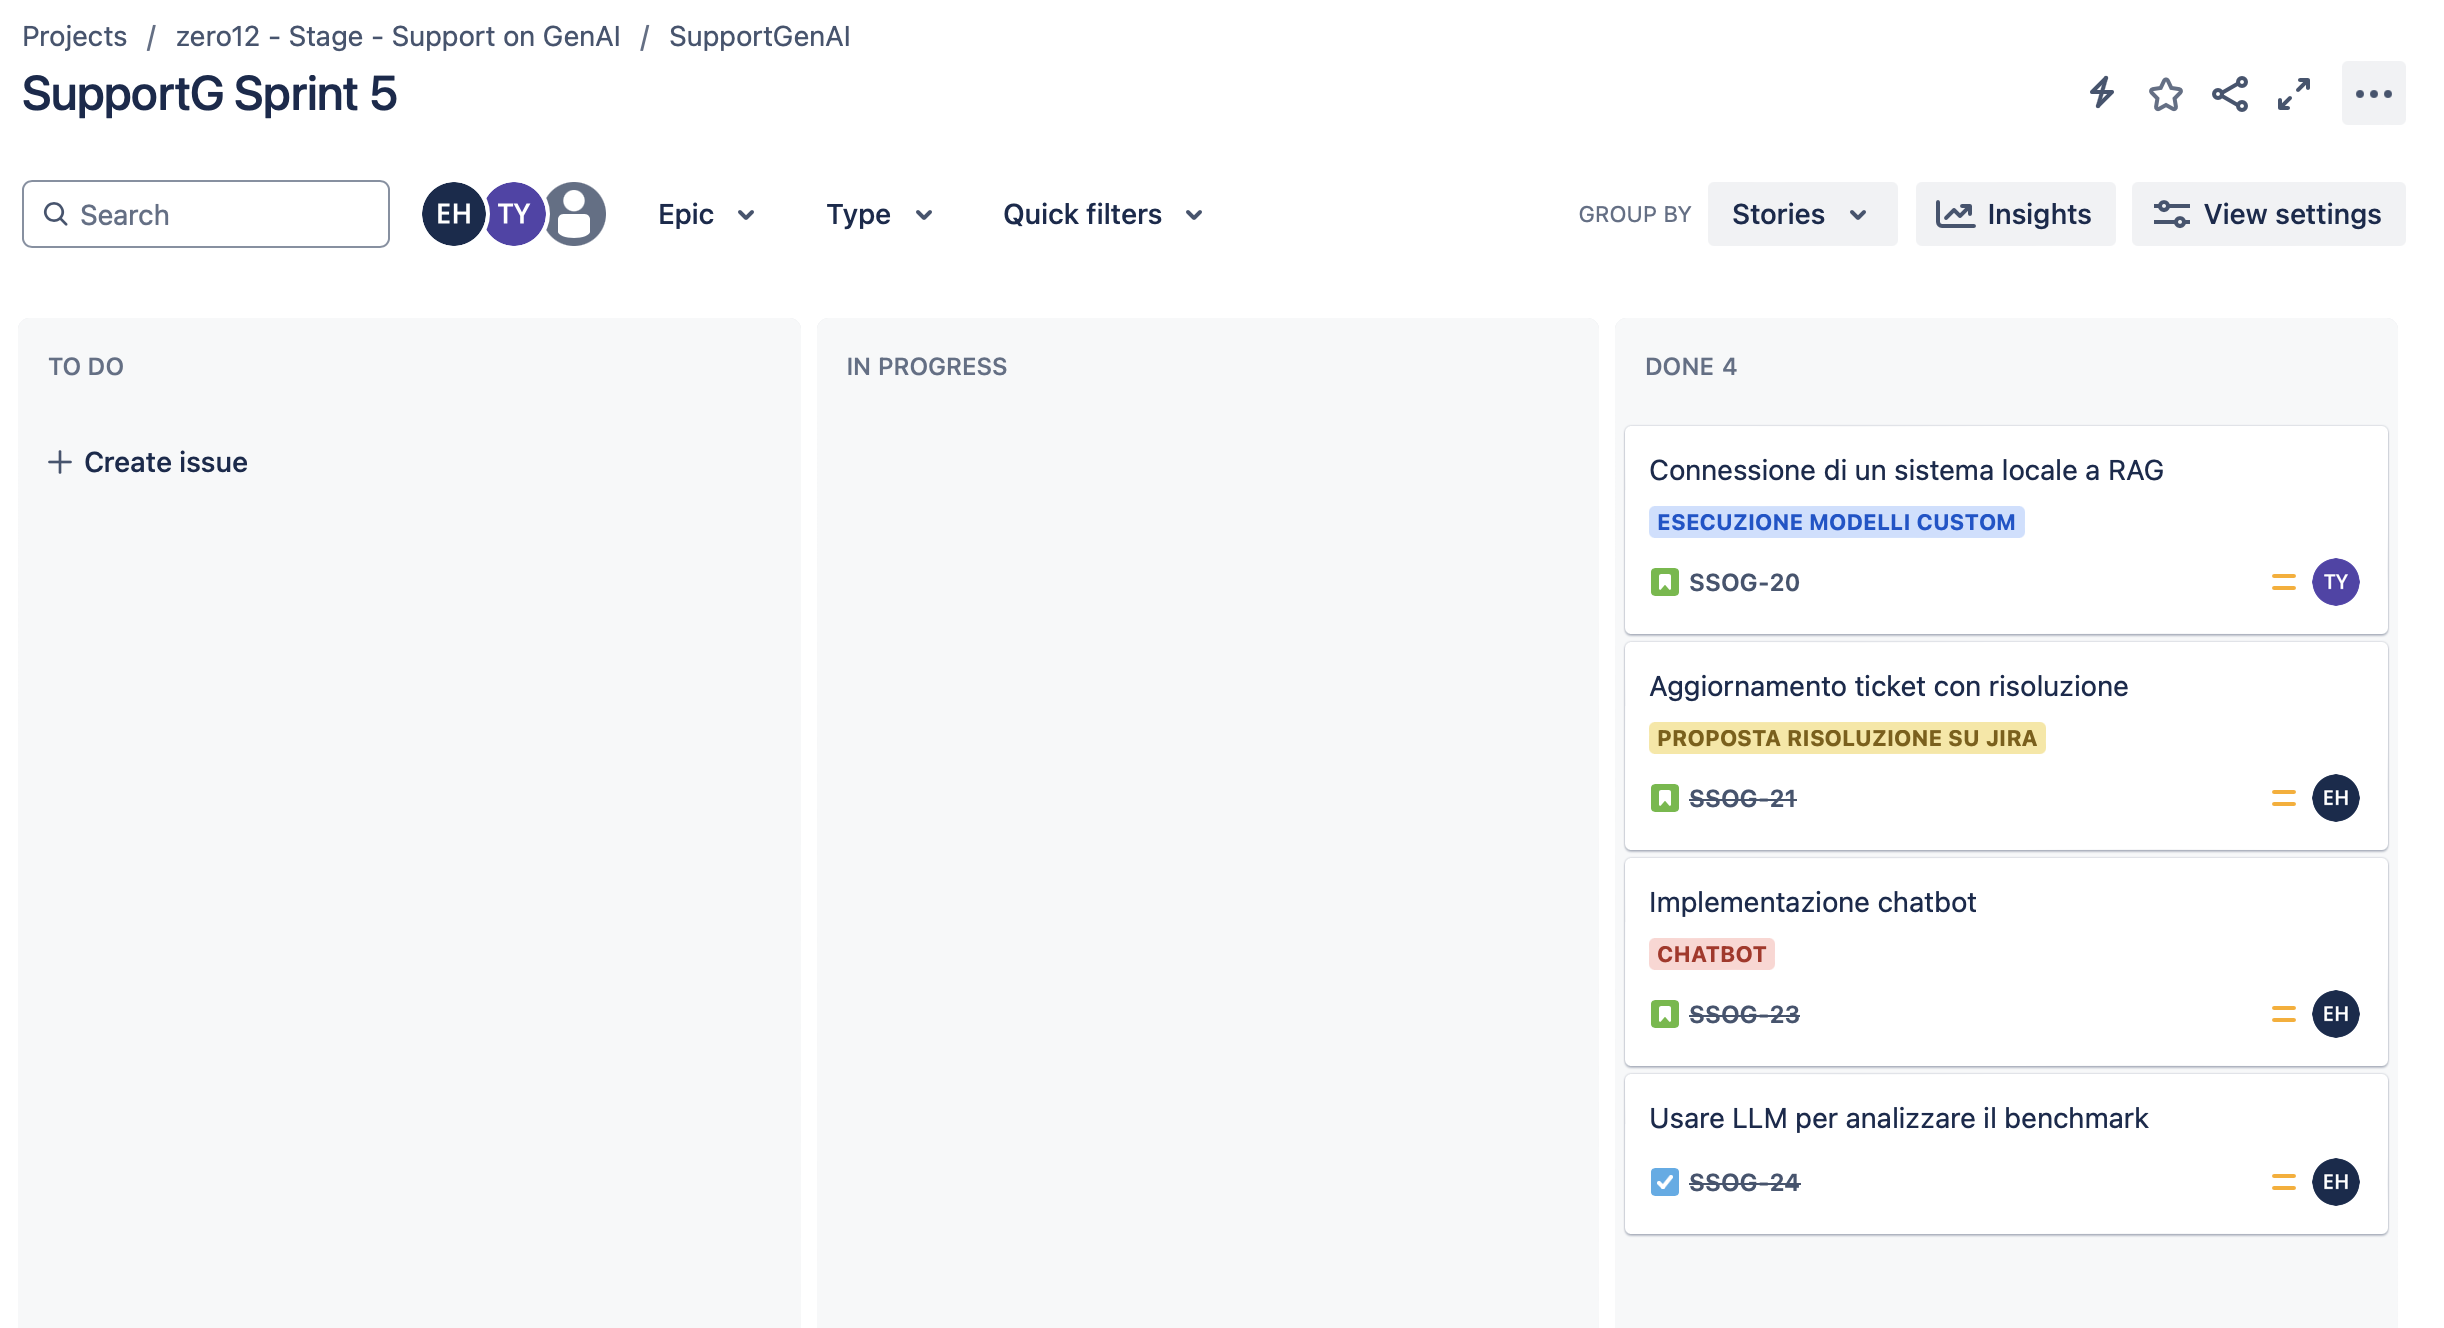
\includegraphics[width=0.65\textwidth]{Jira.png}
    \caption{\textit{Board} del quinto \textit{sprint} del progetto di \textit{stage}}
    \label{fig:Jira}
\end{figure}
\subsubsection{Visual Studio Code}
Visual Studio Code è un \textit{editor} di codice sorgente sviluppato da Microsoft che permette la scrittura di codice in diversi linguaggi di programmazione.
\begin{figure}[H]
    \centering
    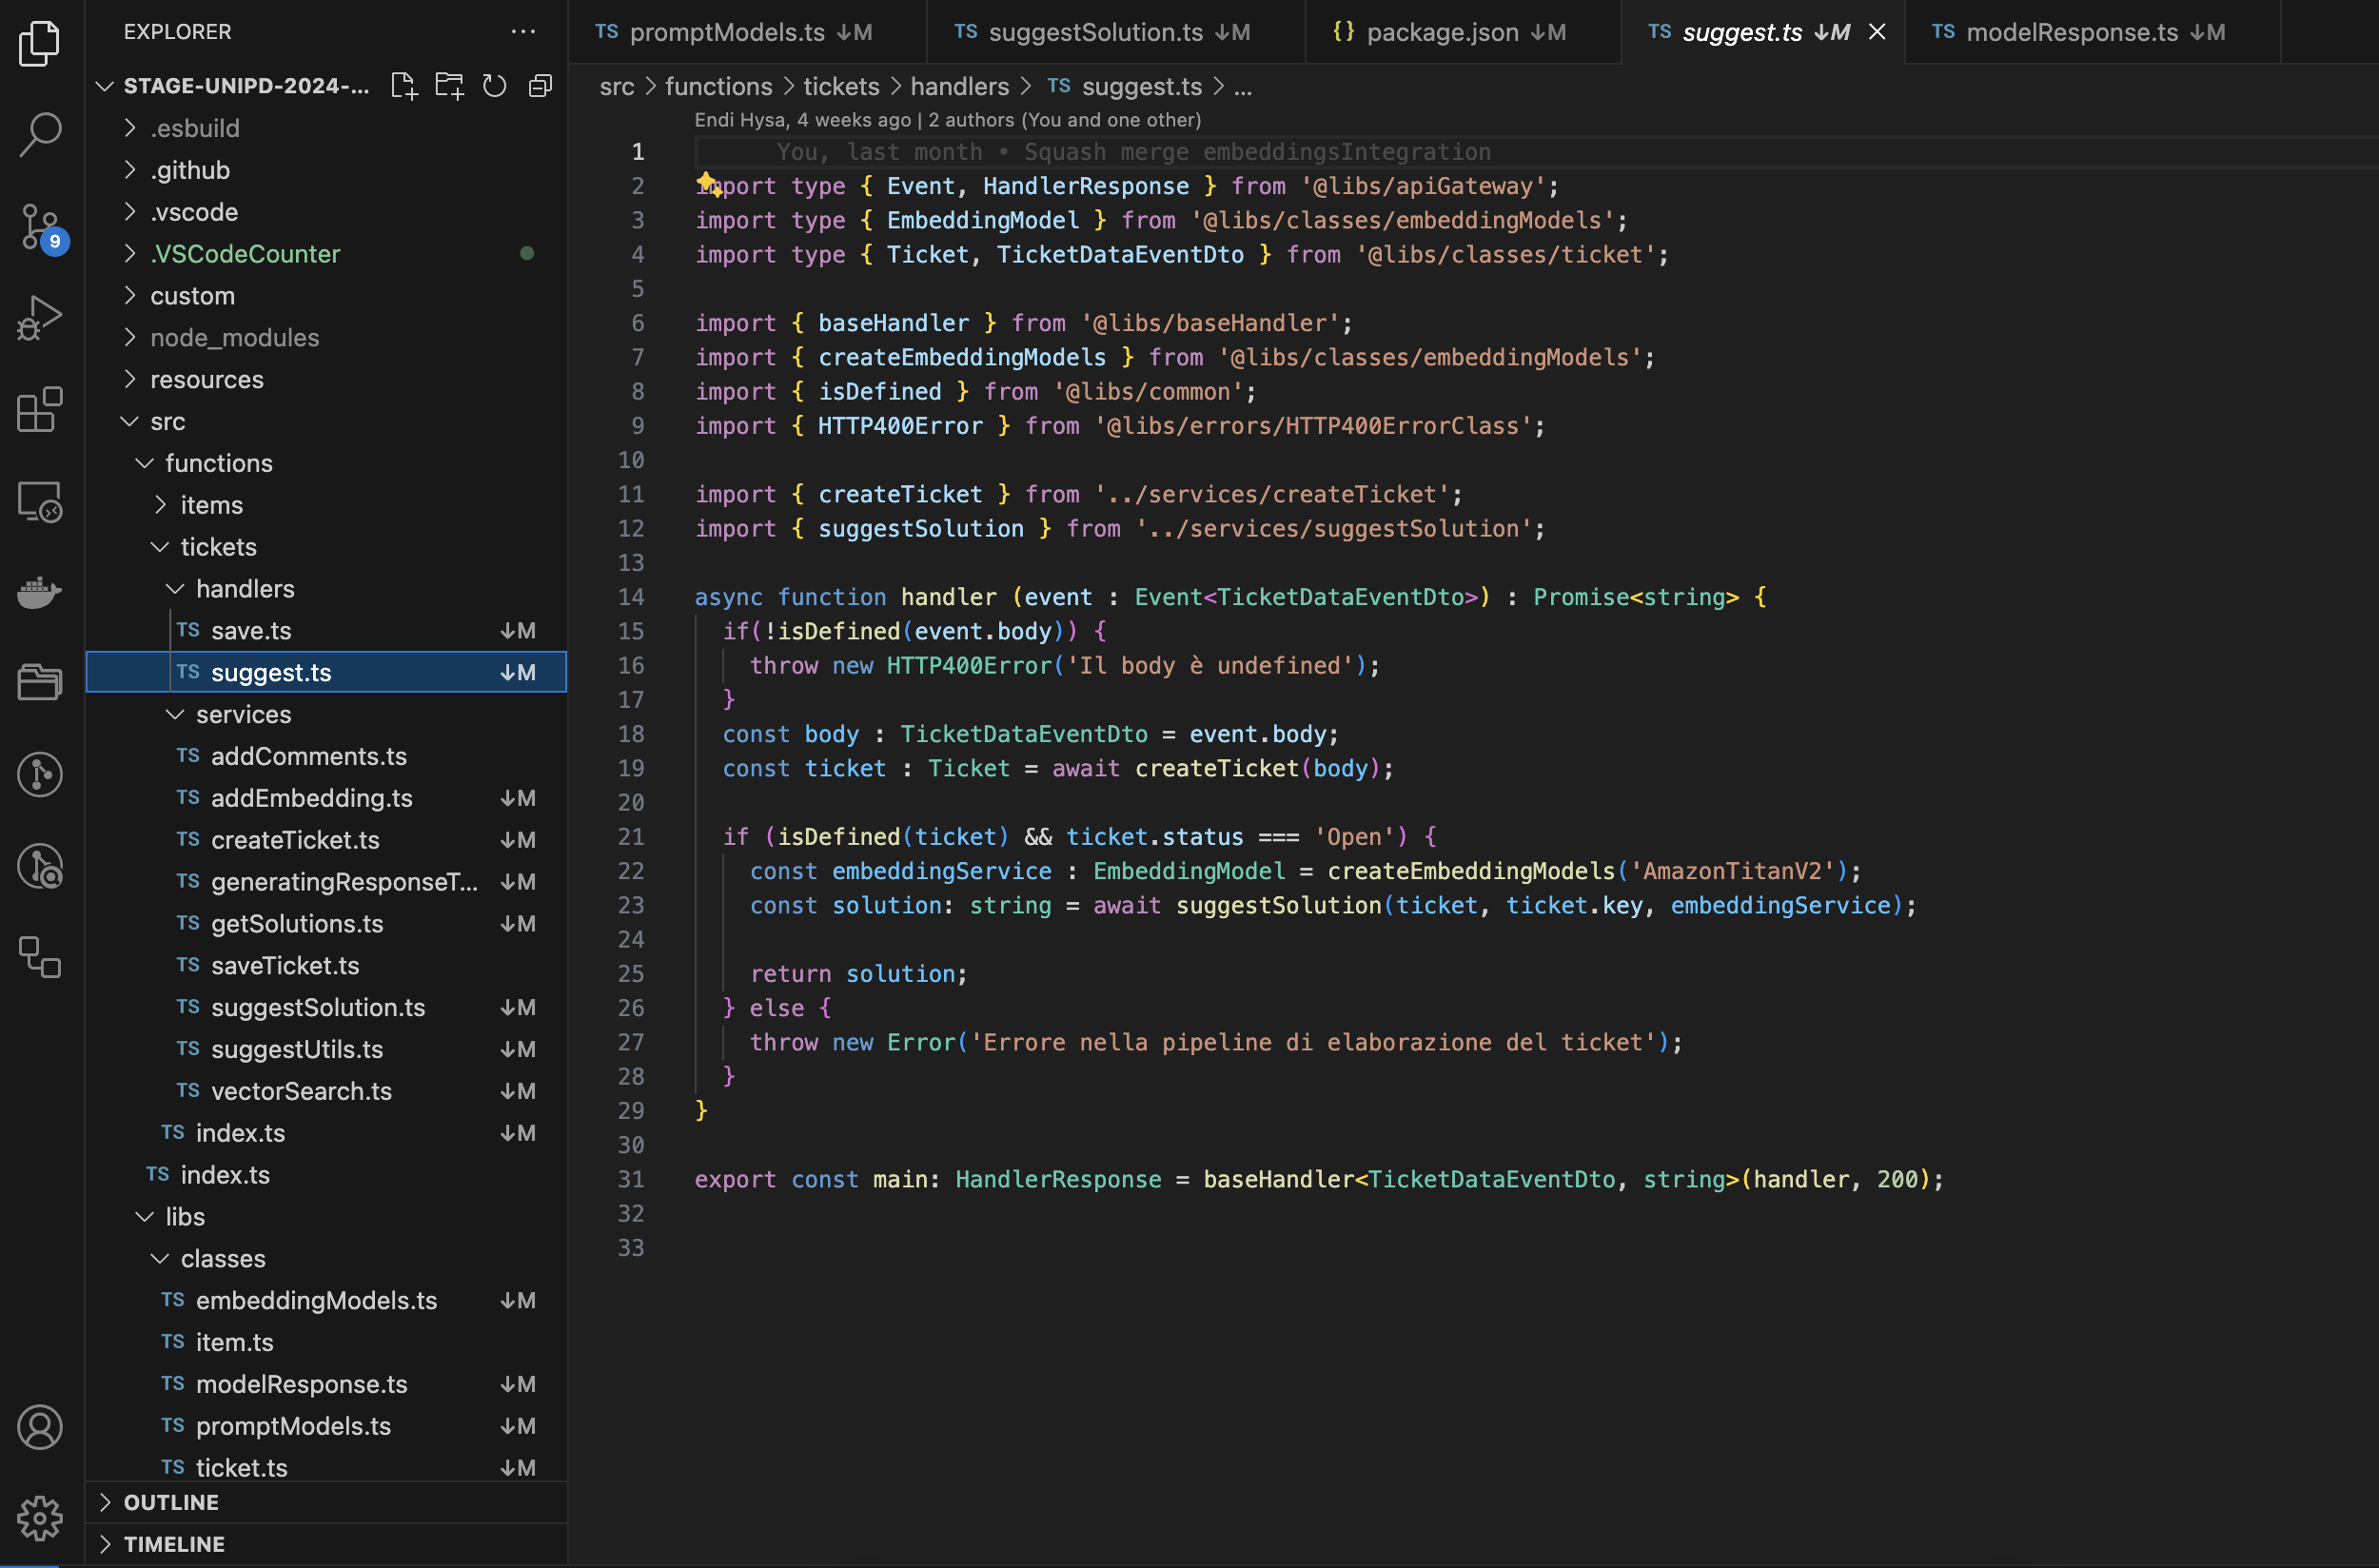
\includegraphics[width=0.65\textwidth]{VsCode.png}
    \caption{Schermata dell'\textit{editor} Visual Studio Code con codice Typescript}
    \label{fig:VsCode}
\end{figure}
\subsubsection{Github}
Github è una piattaforma \textit{web} che permette il versionamento del codice sorgente tramite il sistema di controllo di versione Git. 
Grazie a questo strumento, è possibile creare \textit{repositories} in cui salvare il codice sorgente del progetto. 
È possibile suddividere il progetto in \textit{branch} ed assegnare ad ogni \textit{branch} una \textit{task} da svolgere. Una volta completata la \textit{task}, il \textit{branch} viene unito al \textit{branch} principale tramite una \textit{pull request}. 
Tramite questa pratica è possibile revisionare il codice sorgente prodotto e garantire che il codice prodotto sia conforme alla qualità richiesta.
\begin{figure}[H]
    \centering
    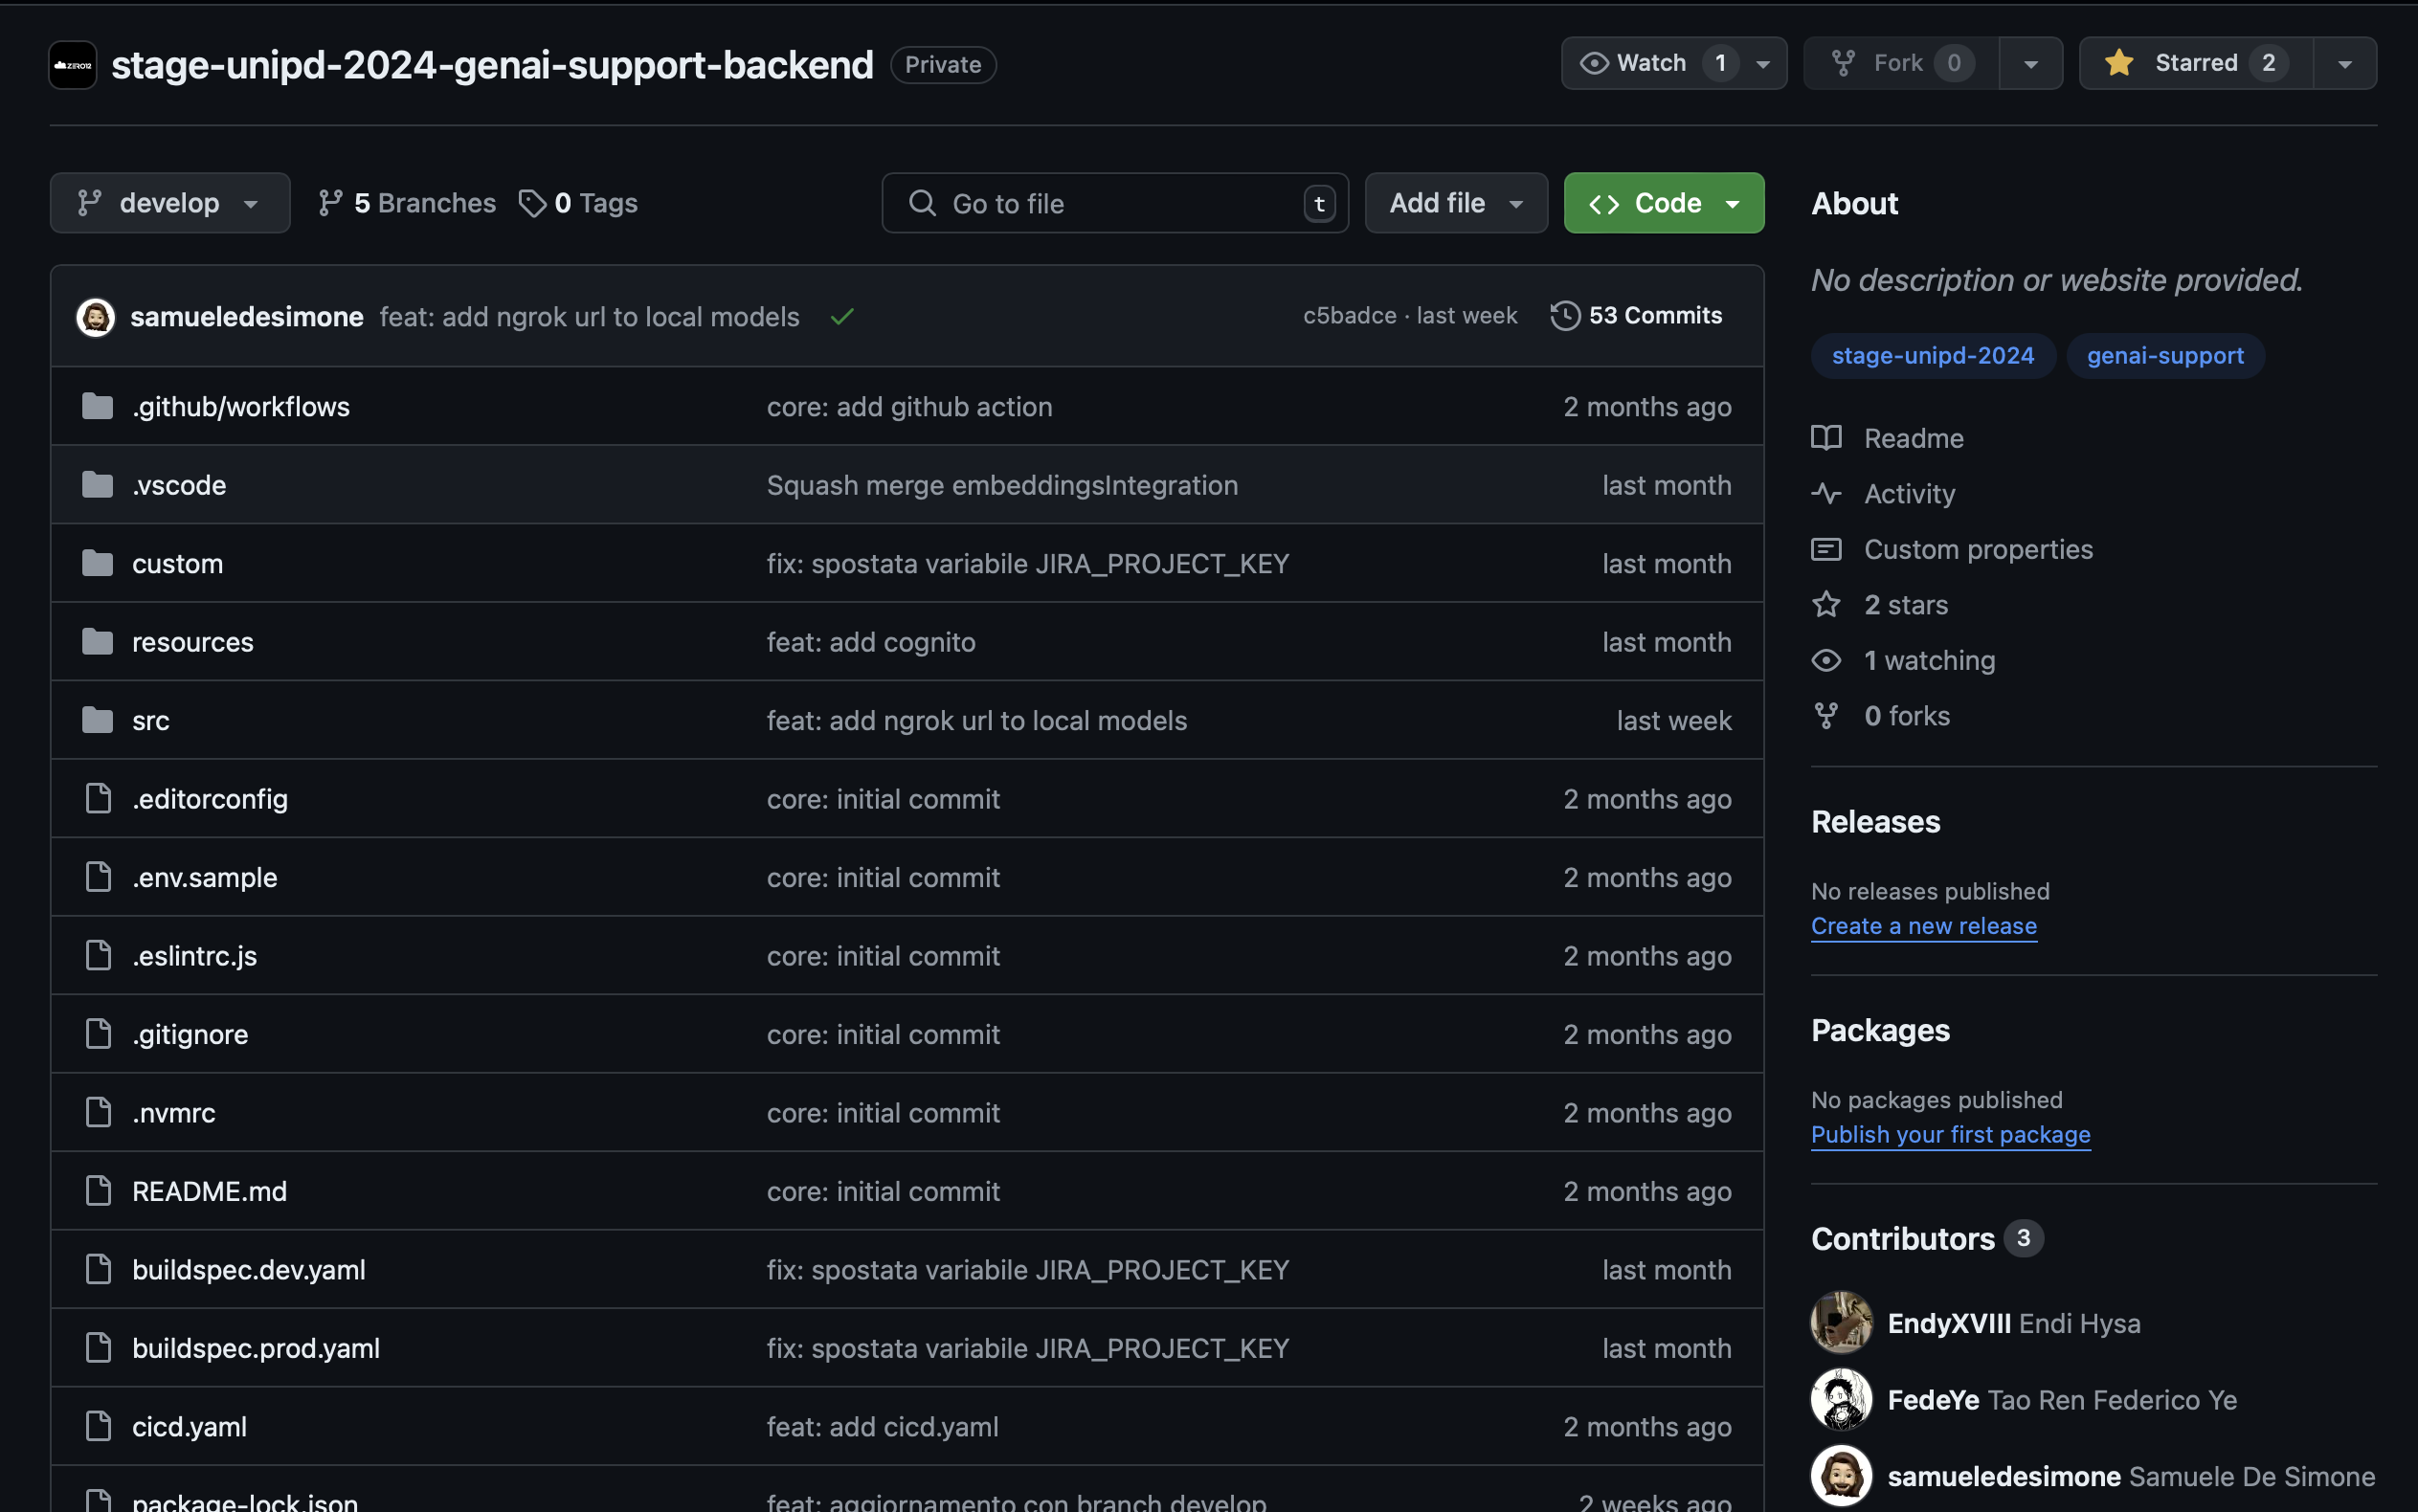
\includegraphics[width=0.65\textwidth]{github.png}
    \caption{Schermata del \textit{repository} Github del progetto di \textit{stage}}
    \label{fig:Github}
\end{figure}
\subsubsection{Slack}
Slack è una piattaforma di messaggistica istantanea utilizzata nell'ambito lavorativo per la comunicazione interna tra i membri del \textit{team}.
Si possono creare canali di comunicazione dedicati a specifici argomenti. In ambito aziendale, viene creato un canale dedicato ad ogni progetto in modo da poter permettere una comunicazione più efficace tra i membri del \textit{team} di lavoro.
Nel caso del mio progetto di \textit{stage} è stato creato un canale dedicato al progetto assieme al mio \textit{tutor} aziendale ed un altra figura per aiutarmi in caso di problematiche.
\begin{figure}[H]
    \centering
    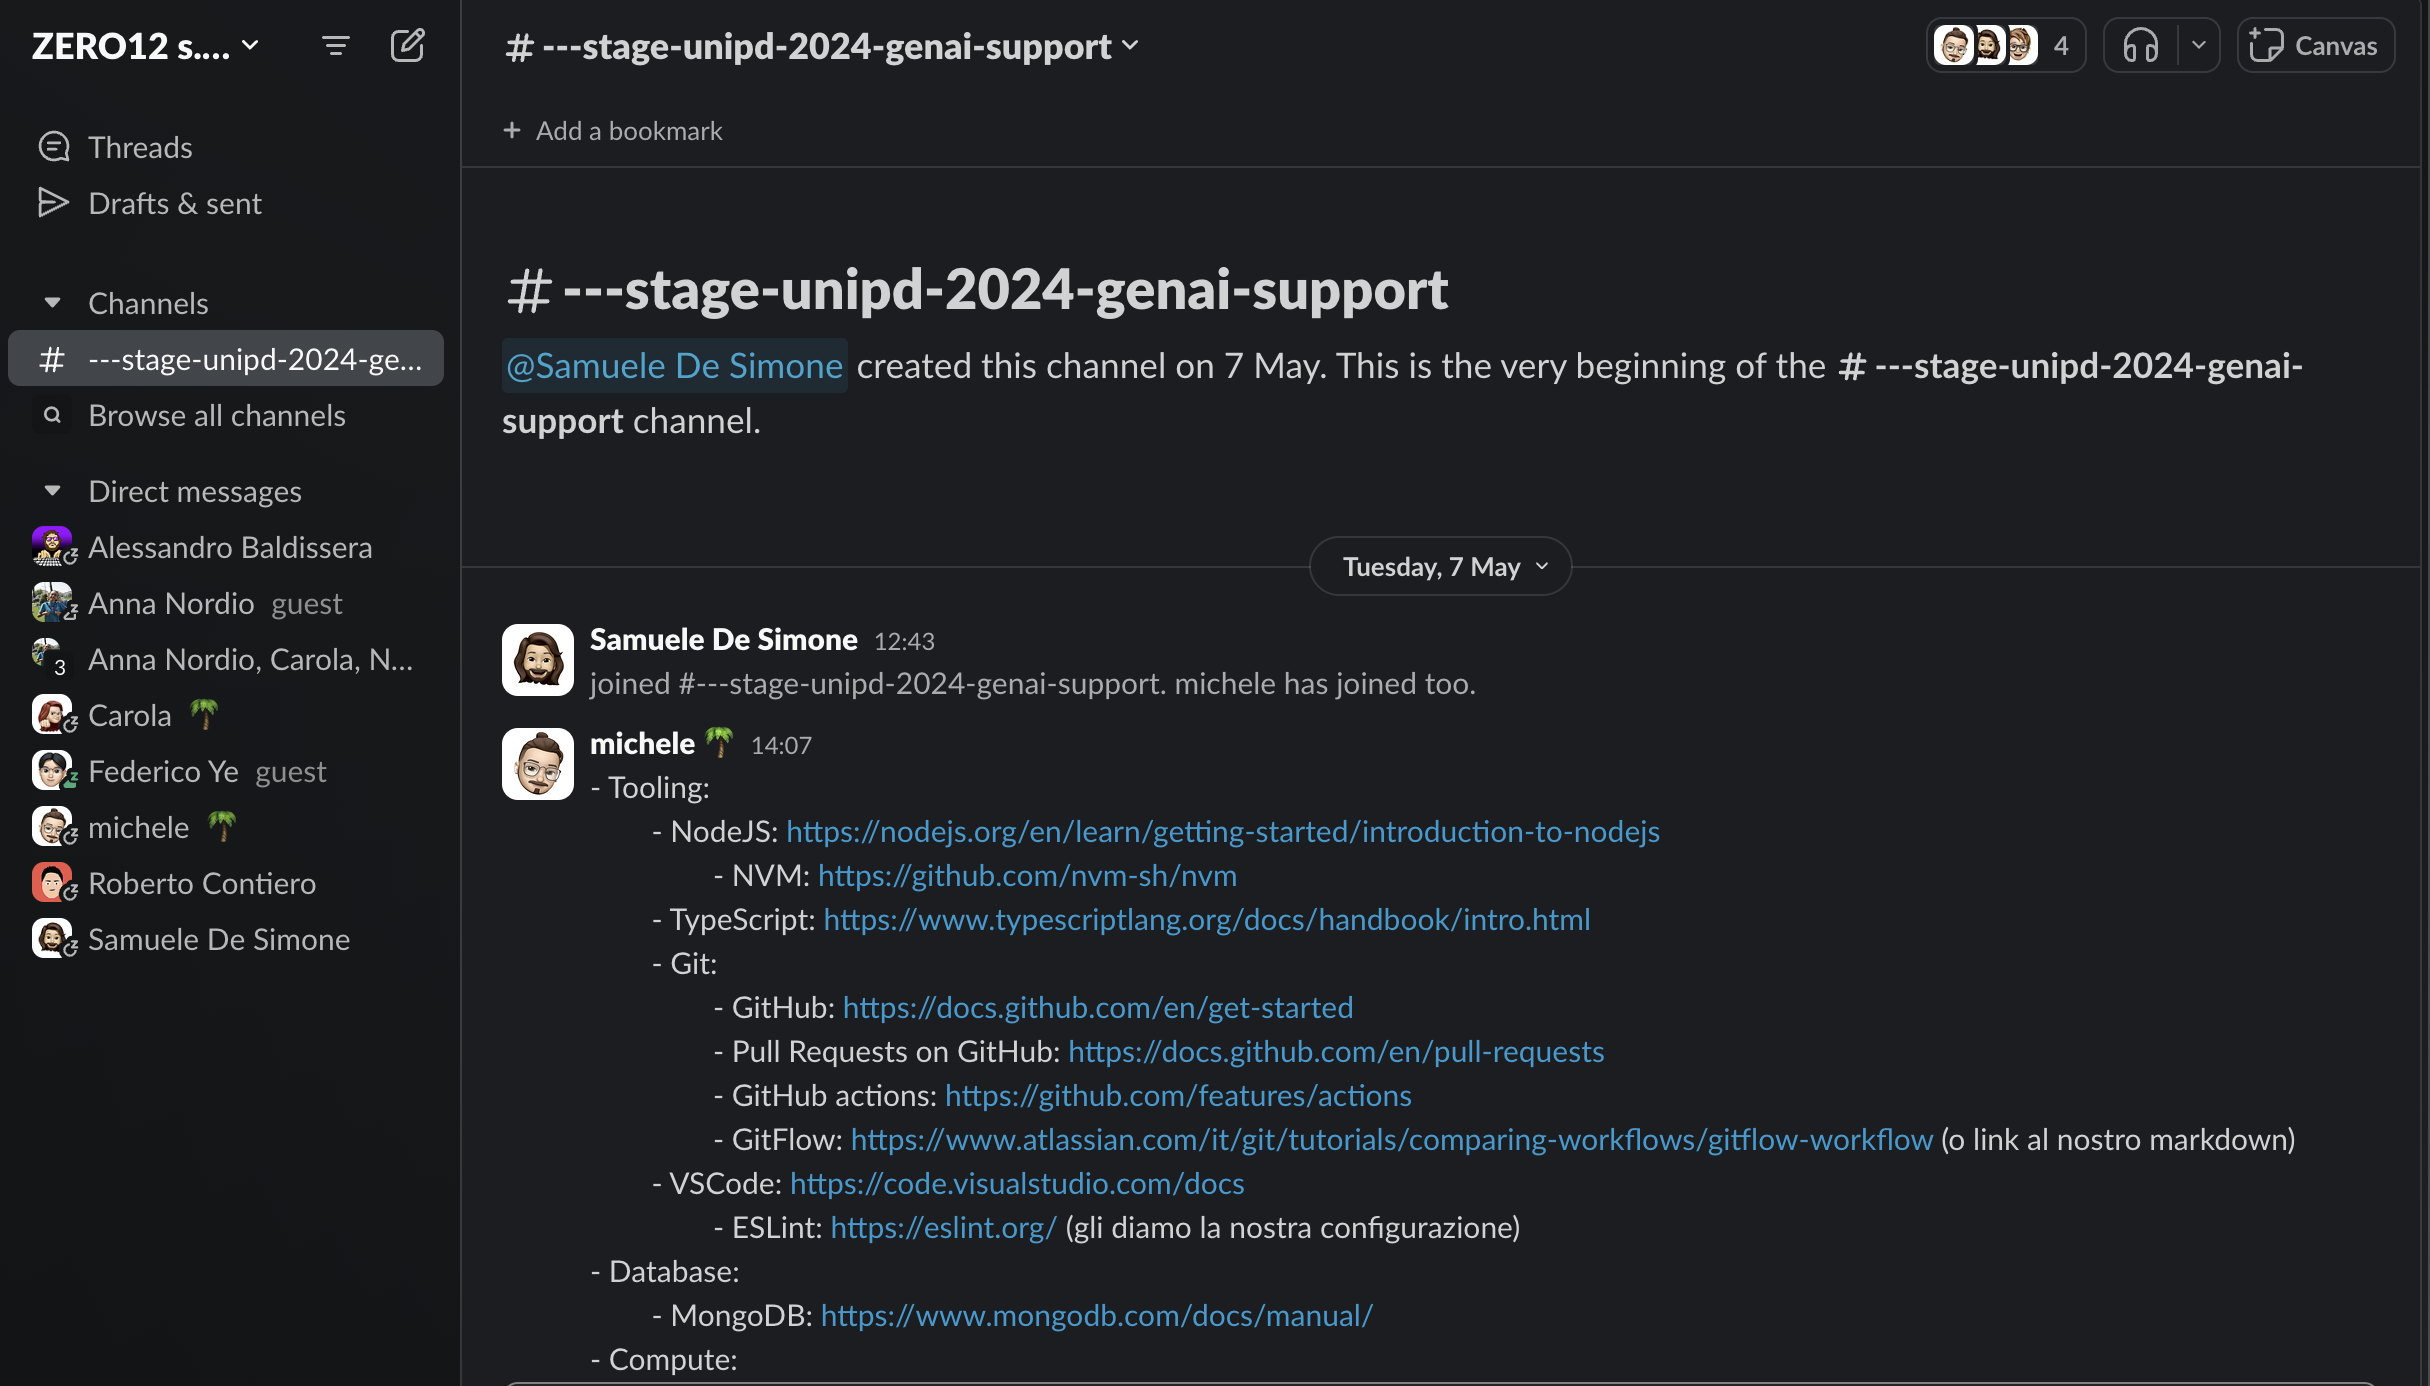
\includegraphics[width=0.65\textwidth]{slack.png}
    \caption{Schermata del canale dedicato al progetto di \textit{stage}}
    \label{fig:Slack}
\end{figure}

\section{Tecnologie utilizzate}
\subsection{Tecnologie di sviluppo}
\subsubsection{Typescript}
TypeScript è un linguaggio di programmazione sviluppato da Microsoft, noto per essere un \textit{superset} di JavaScript che introduce tipi statici opzionali. La scelta di TypeScript per lo sviluppo del progetto è motivata dal suo sistema di tipizzazione statica, che consente di individuare errori di programmazione durante la fase di sviluppo.
migliorando così la robustezza e la manutenibilità del codice.

\subsubsection{Python}
\textit{Python} è un linguaggio di programmazione ad alto livello, interpretato e multiparadigma. Il suo utilizzo è motivato dalla sua semplicità, flessibilità e dalla vasta gamma di librerie disponibili per la realizzazione di progetti di vario genere.
\subsubsection{Node.js}
Node.js è un ambiente \textit{runtime} di Javascript che consente di eseguire codice Javascript al di fuori di un \textit{browser}. È basato sul motore JavaScript V8 sviluppato da \textit{Google}. Viene utilizzato per la creazione di applicazioni \textit{web} \textit{server-side} in modo efficiente e scalabile.
\subsubsection{MongoDB}
MongoDB è un \textit{database} non relazionale (\textit{NoSQL}) dove i dati non vengono strutturati in tabelle con uno schema preciso, ma vengono raggruppati in documenti dove la struttura dei dati può variare da documento a documento.  
\begin{figure}[H]
    \centering
    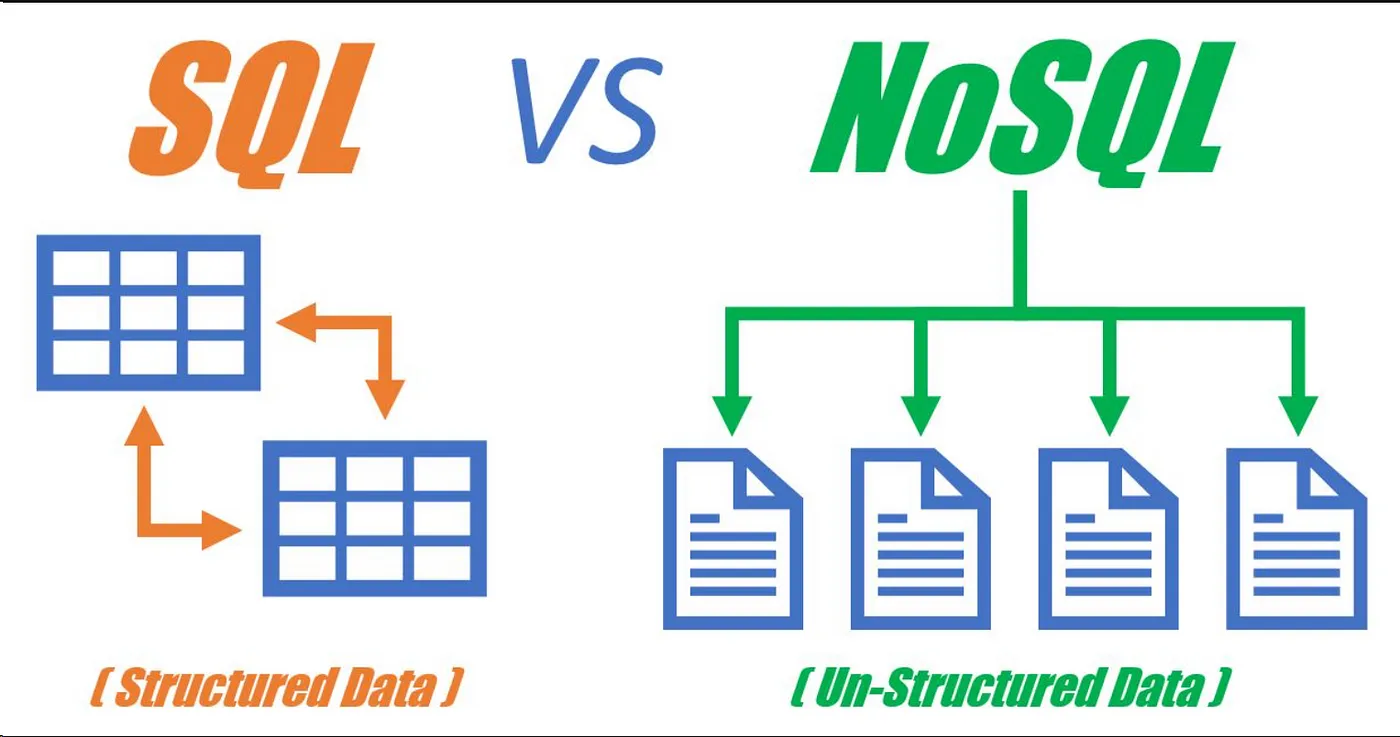
\includegraphics[width=0.65\textwidth]{sqlvsnosql.png}
    \caption{Differenza tra la struttura di un \textit{database} relazionale e un \textit{database} non relazionale}
    \small \textbf{Fonte:} \href{https://naveen-metta.medium.com/decoding-the-database-dilemma-sql-vs-nosql-in-system-design-876e21f4a58c}{medium.com}
    \label{fig:sql-vs-nosql}
\end{figure} 

\subsubsection{Serverless framework}
Il Serverless \textit{framework} è un \textit{framework} che permette la creazione di \gls{api}, un \textit{software} che definisce come due parti (applicazione \textit{client} e \textit{server}) comunicano tra loro usando richieste e risposte, su infrastuttura \gls{awsg}, che permette la definizione di funzioni \textit{lambda} con i relativi \textit{trigger} di invocazione.
Permette inoltre il \textit{deploy} nel \textit{cloud} attraverso un semplice comando che carica il codice sorgente e configura l'architettura in modo automatico. Supporta diversi \textit{plugin} che permettono l'utilizzo di altri servizi offerti da \gls{awsg}.
\begin{figure}[H]
    \centering
    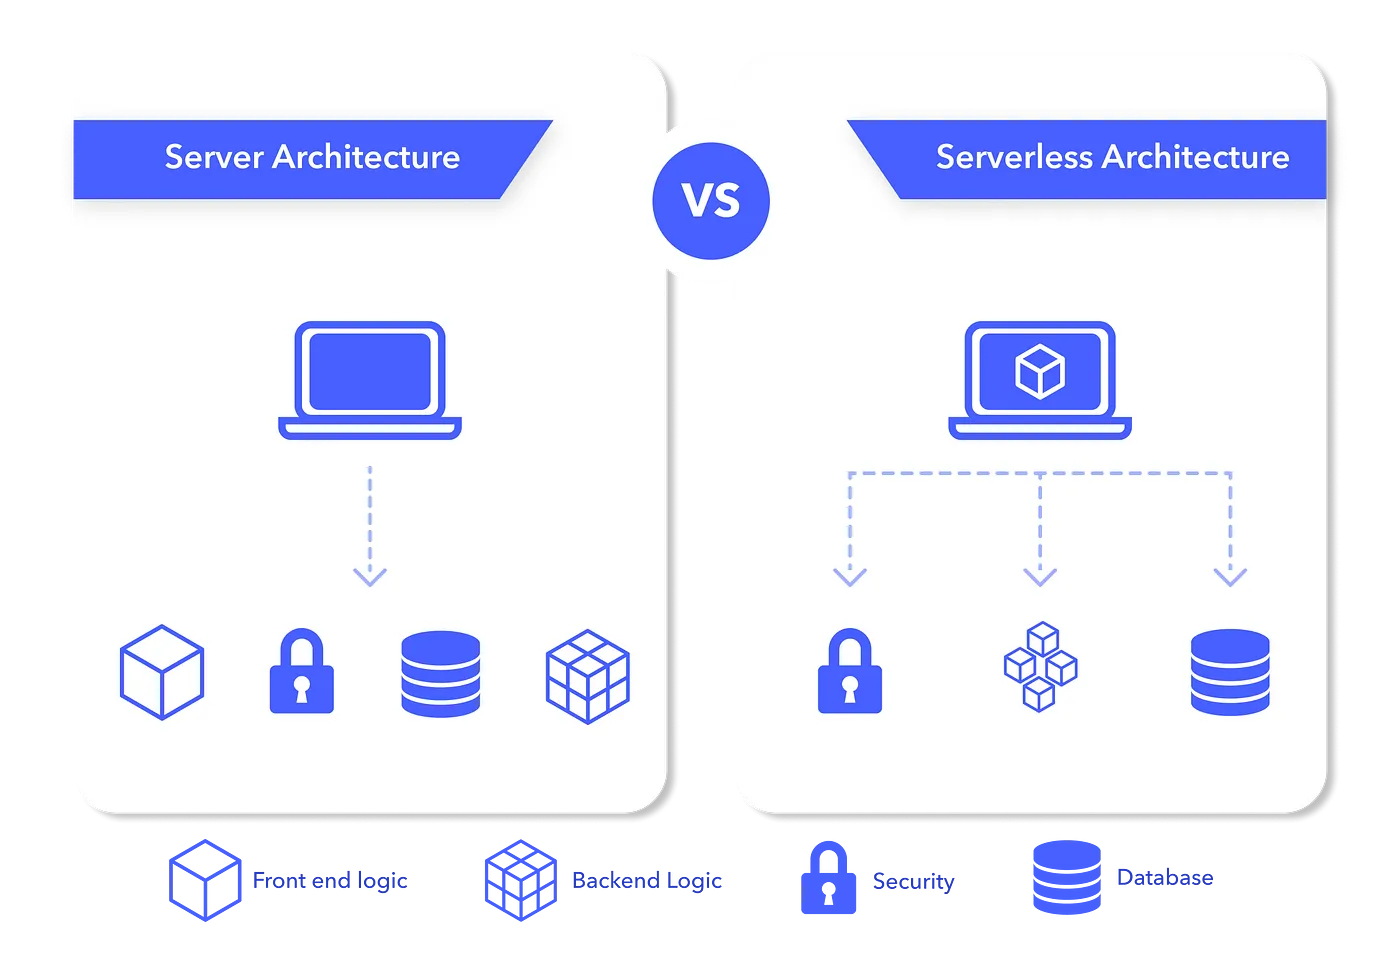
\includegraphics[width=0.65\textwidth]{serverless.png}
    \caption{Confronto tra un'architettura tradizionale e una architettura \textit{\gls{serverlessg}}}
    \small \textbf{Fonte:} \href{https://medium.com/canonichq/server-v-s-serverless-architecture-bf3cdab28174}{medium.com}
    \label{fig:Serverless}
\end{figure} 
\noindent
Come mostrato nella figura \ref{fig:Serverless}, l'architettura \textit{\gls{serverlessg}} permette all'utente di non doversi preoccupare della gestione dell'infrastruttura sottostante, in quanto viene gestita automaticamente dal fornitore del servizio. Nella controparte dell'architettura tradizionale, l'utente deve gestire l'infrastruttura sottostante.
\subsubsection{Streamlit}
Streamlit è un \textit{framework open-source} che permette la creazione di applicazioni \textit{web} per la visualizzazione di dati in modo rapido e semplice.
Con l'utilizzo del seguente \textit{framework} si possono trasformare \textit{script} Python in applicazioni \textit{web} interattive.
\begin{figure}[H]
    \centering
    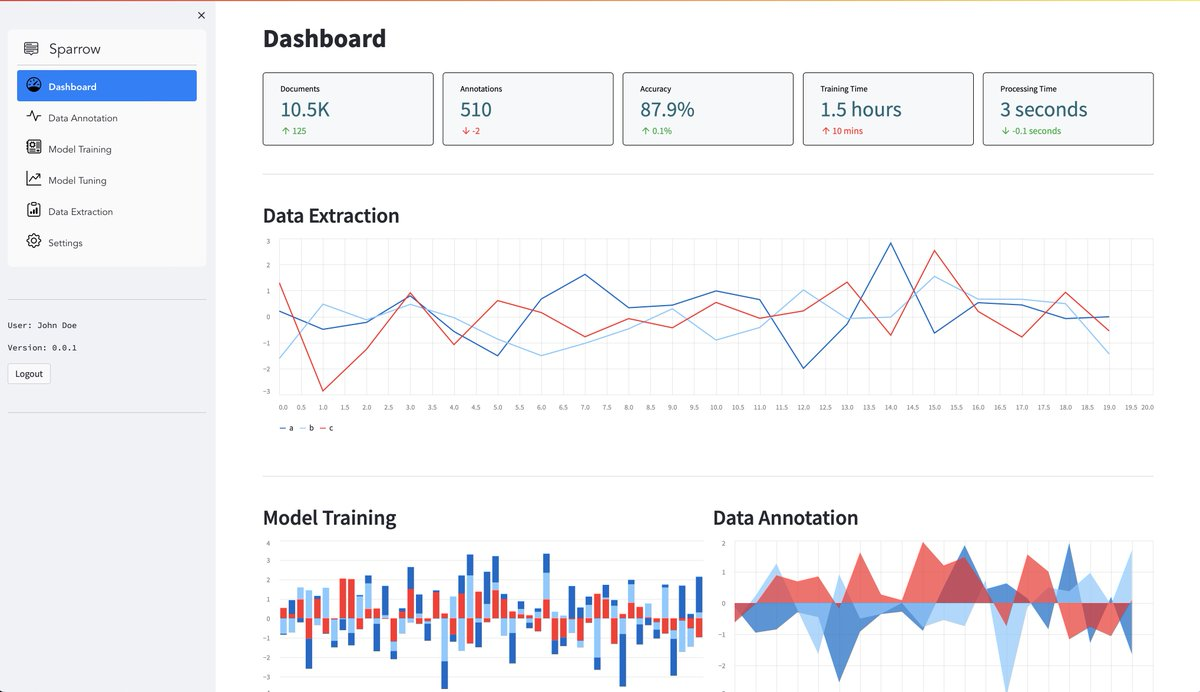
\includegraphics[width=0.65\textwidth]{streamlit.png}
    \caption{Esempio di applicazione \textit{web} creata con il \textit{framework} Streamlit}
    \small \textbf{Fonte:} \href{https://streamlit.io}{streamlit.io}
    \label{fig:Streamlit}
\end{figure} 

\subsubsection {Servizi AWS}
Nella realizzazione del progetto di \textit{stage} sono stati utilizzati diversi servizi offerti da \gls{awsg}. I servizi principali utilizzati sono:
\begin{itemize}
    \item \textbf{AWS Lambda}: servizio che permette l'esecuzione di codice senza la necessitò di dover gestire \textit{server} sottostanti. Sono autoscalabili in base al carico di lavoro. Generalmente sono funzioni che seguono il \textit{Simple Responsability Principle}.
    \item \textbf{AWS Bedrock}: servizio che permette l'utilizzo di vari modelli di \textit{machine learning}, utilizzabili tramite chiamata \gls{api}.
    \item \textbf{AWS API Gateway}: servizio che permette la creazione, la pubblicazione, la manutenzione, il monitoraggio e la protezione di \gls{api} su larga scala.
\end{itemize}
Alcuni servizi vengono utilizzati per attuare il processo di \gls{ci-cd}, una pratica di sviluppo in cui tutte le modifiche apportate al \textit{software} durante lo sviluppo, vengono integrate e testate automaticamente, in modo da garantire che il codice sia sempre funzionante e pronto per il rilascio.
\subsection{Tecnologie per la validazione del codice}
\subsubsection{ESLint}
ESLint è un \textit{plugin} installato su Visual Studio Code che permette il controllo del codice in fase di scrittura, segnando eventuali errori di sintassi o di stile.
È possibile impostare una configurazione personalizzata (come l'indentazione del codice, la lunghezza delle righe, ecc.), permettendo così di scrivere codice uniforme agli \textit{standard} aziendali.
\begin{figure}[H]
    \centering
    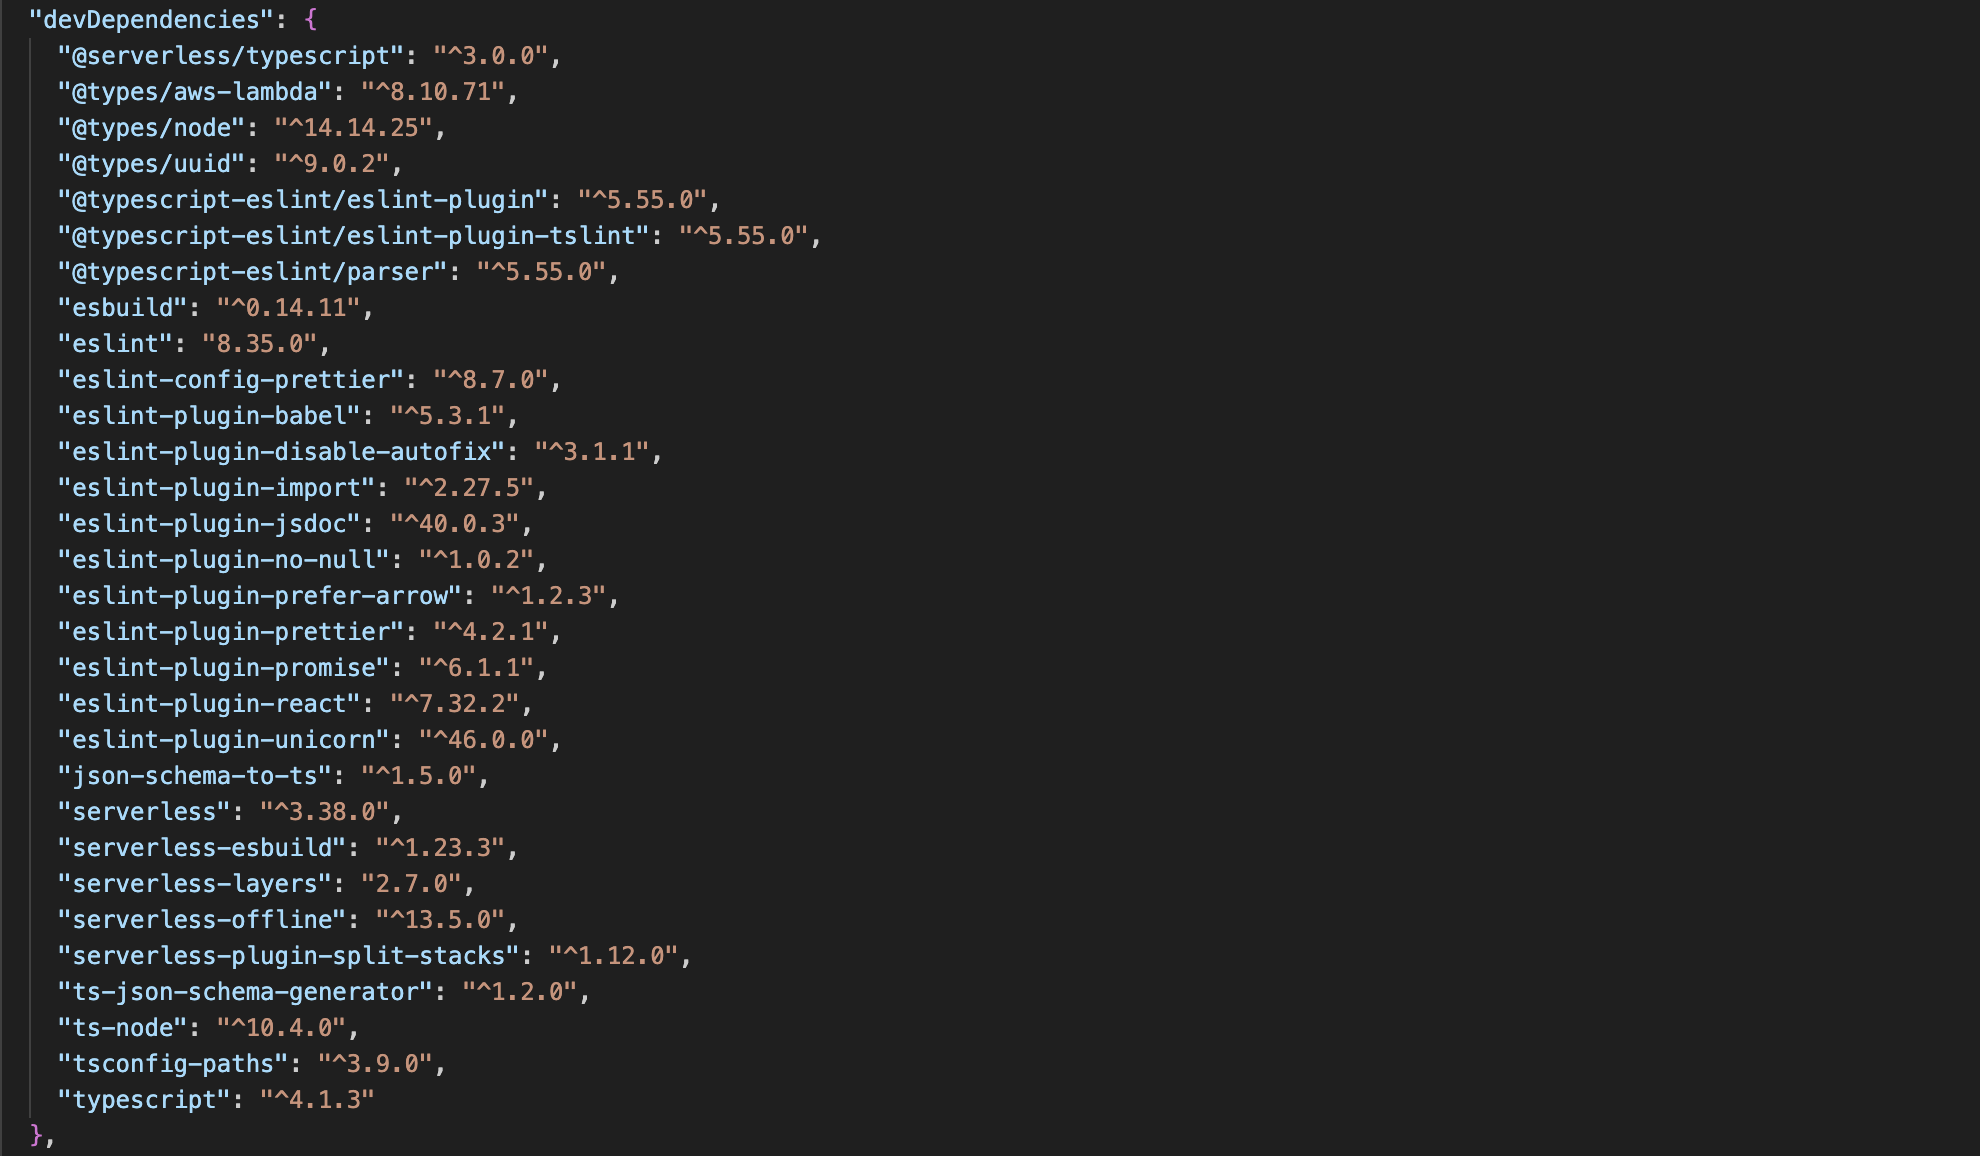
\includegraphics[width=0.65\textwidth]{eslint.png}
    \caption{Esempio di configurazione di ESLint}
    \label{fig:ESlint}
\end{figure} 
\pagebreak
\subsection{Tecnologie di supporto}
\subsubsection{Postman}
Postman è un \textit{software} che permette il salvataggio e il testing di \gls{api} in modo semplice. Offre un'interfaccia intuitiva che permette di organizzare le richieste e generare documentazione delle \gls{api} salvate.
\begin{figure}[H]
    \centering
    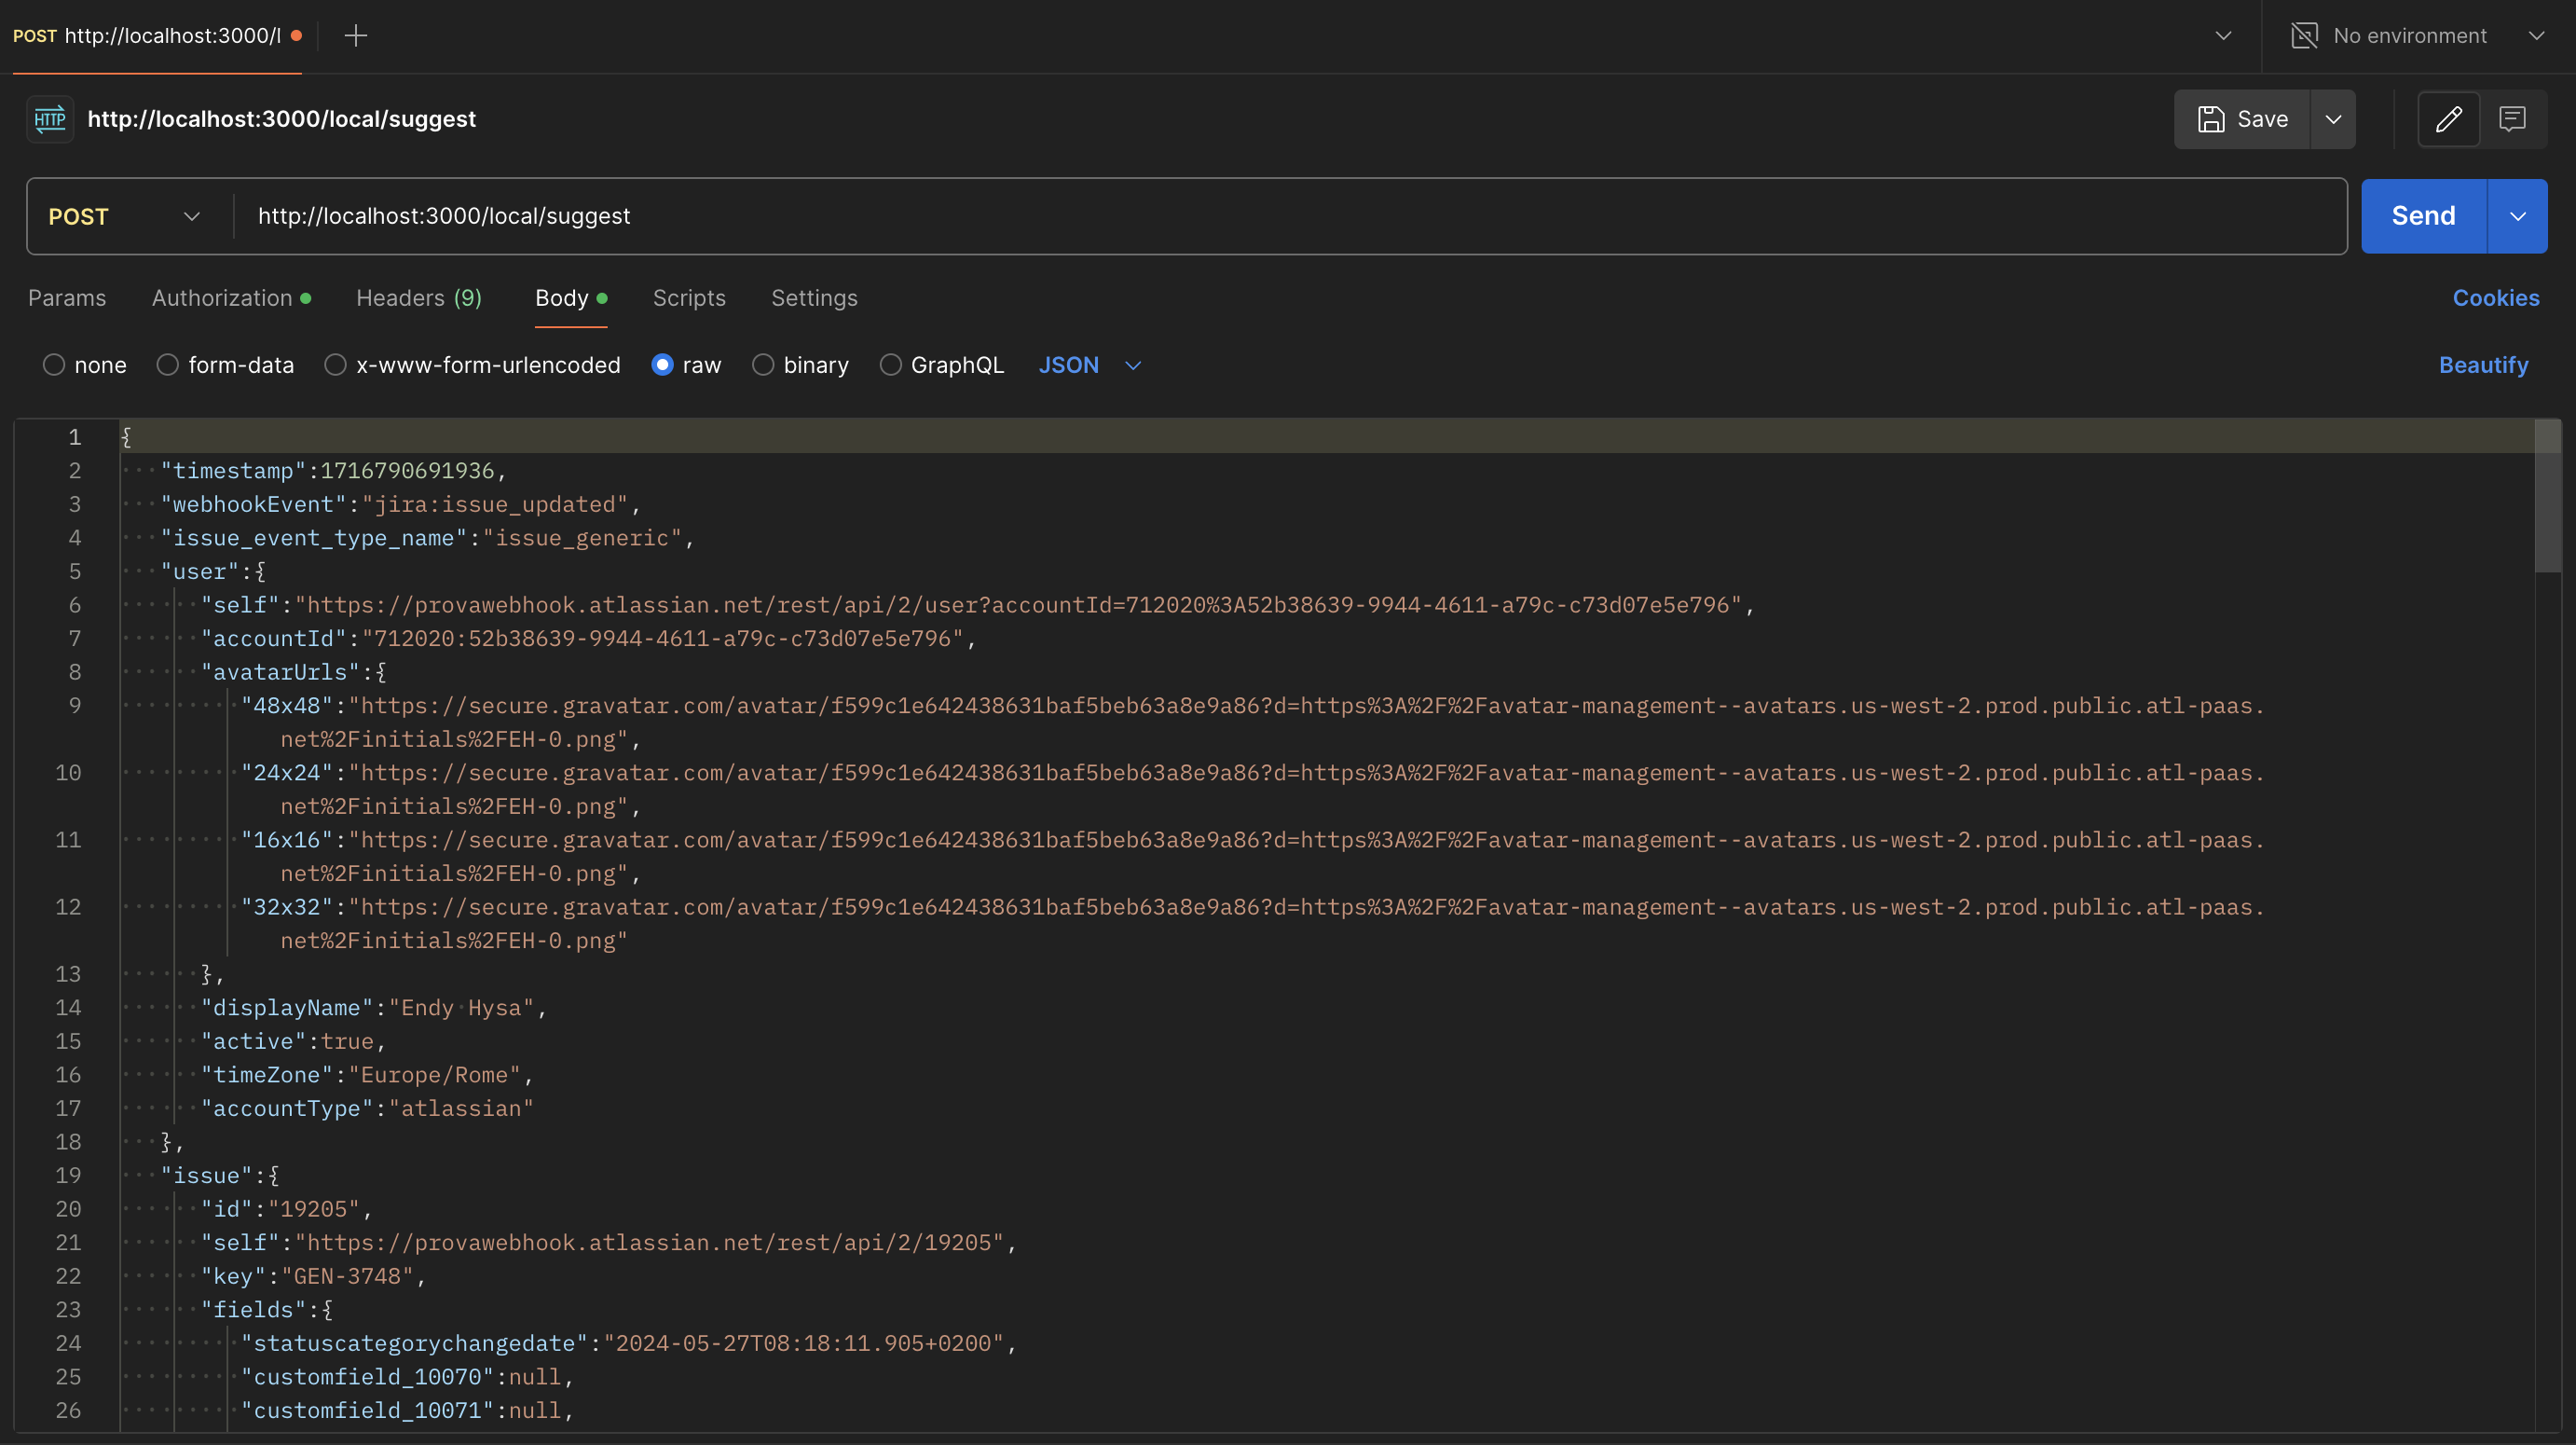
\includegraphics[width=0.65\textwidth]{postman.png}
    \caption{Esempio di API di tipo \textit{POST} su Postman con relativo \textit{body}}
    \label{fig:Postman}
\end{figure} 

\subsubsection{MongoDB Compass}
MongoDB Compass è un \textit{software} che permette la visualizzazione dei documenti salvati nel \textit{database} MongoDB tramite un'interfaccia grafica.
\begin{figure}[H]
    \centering
    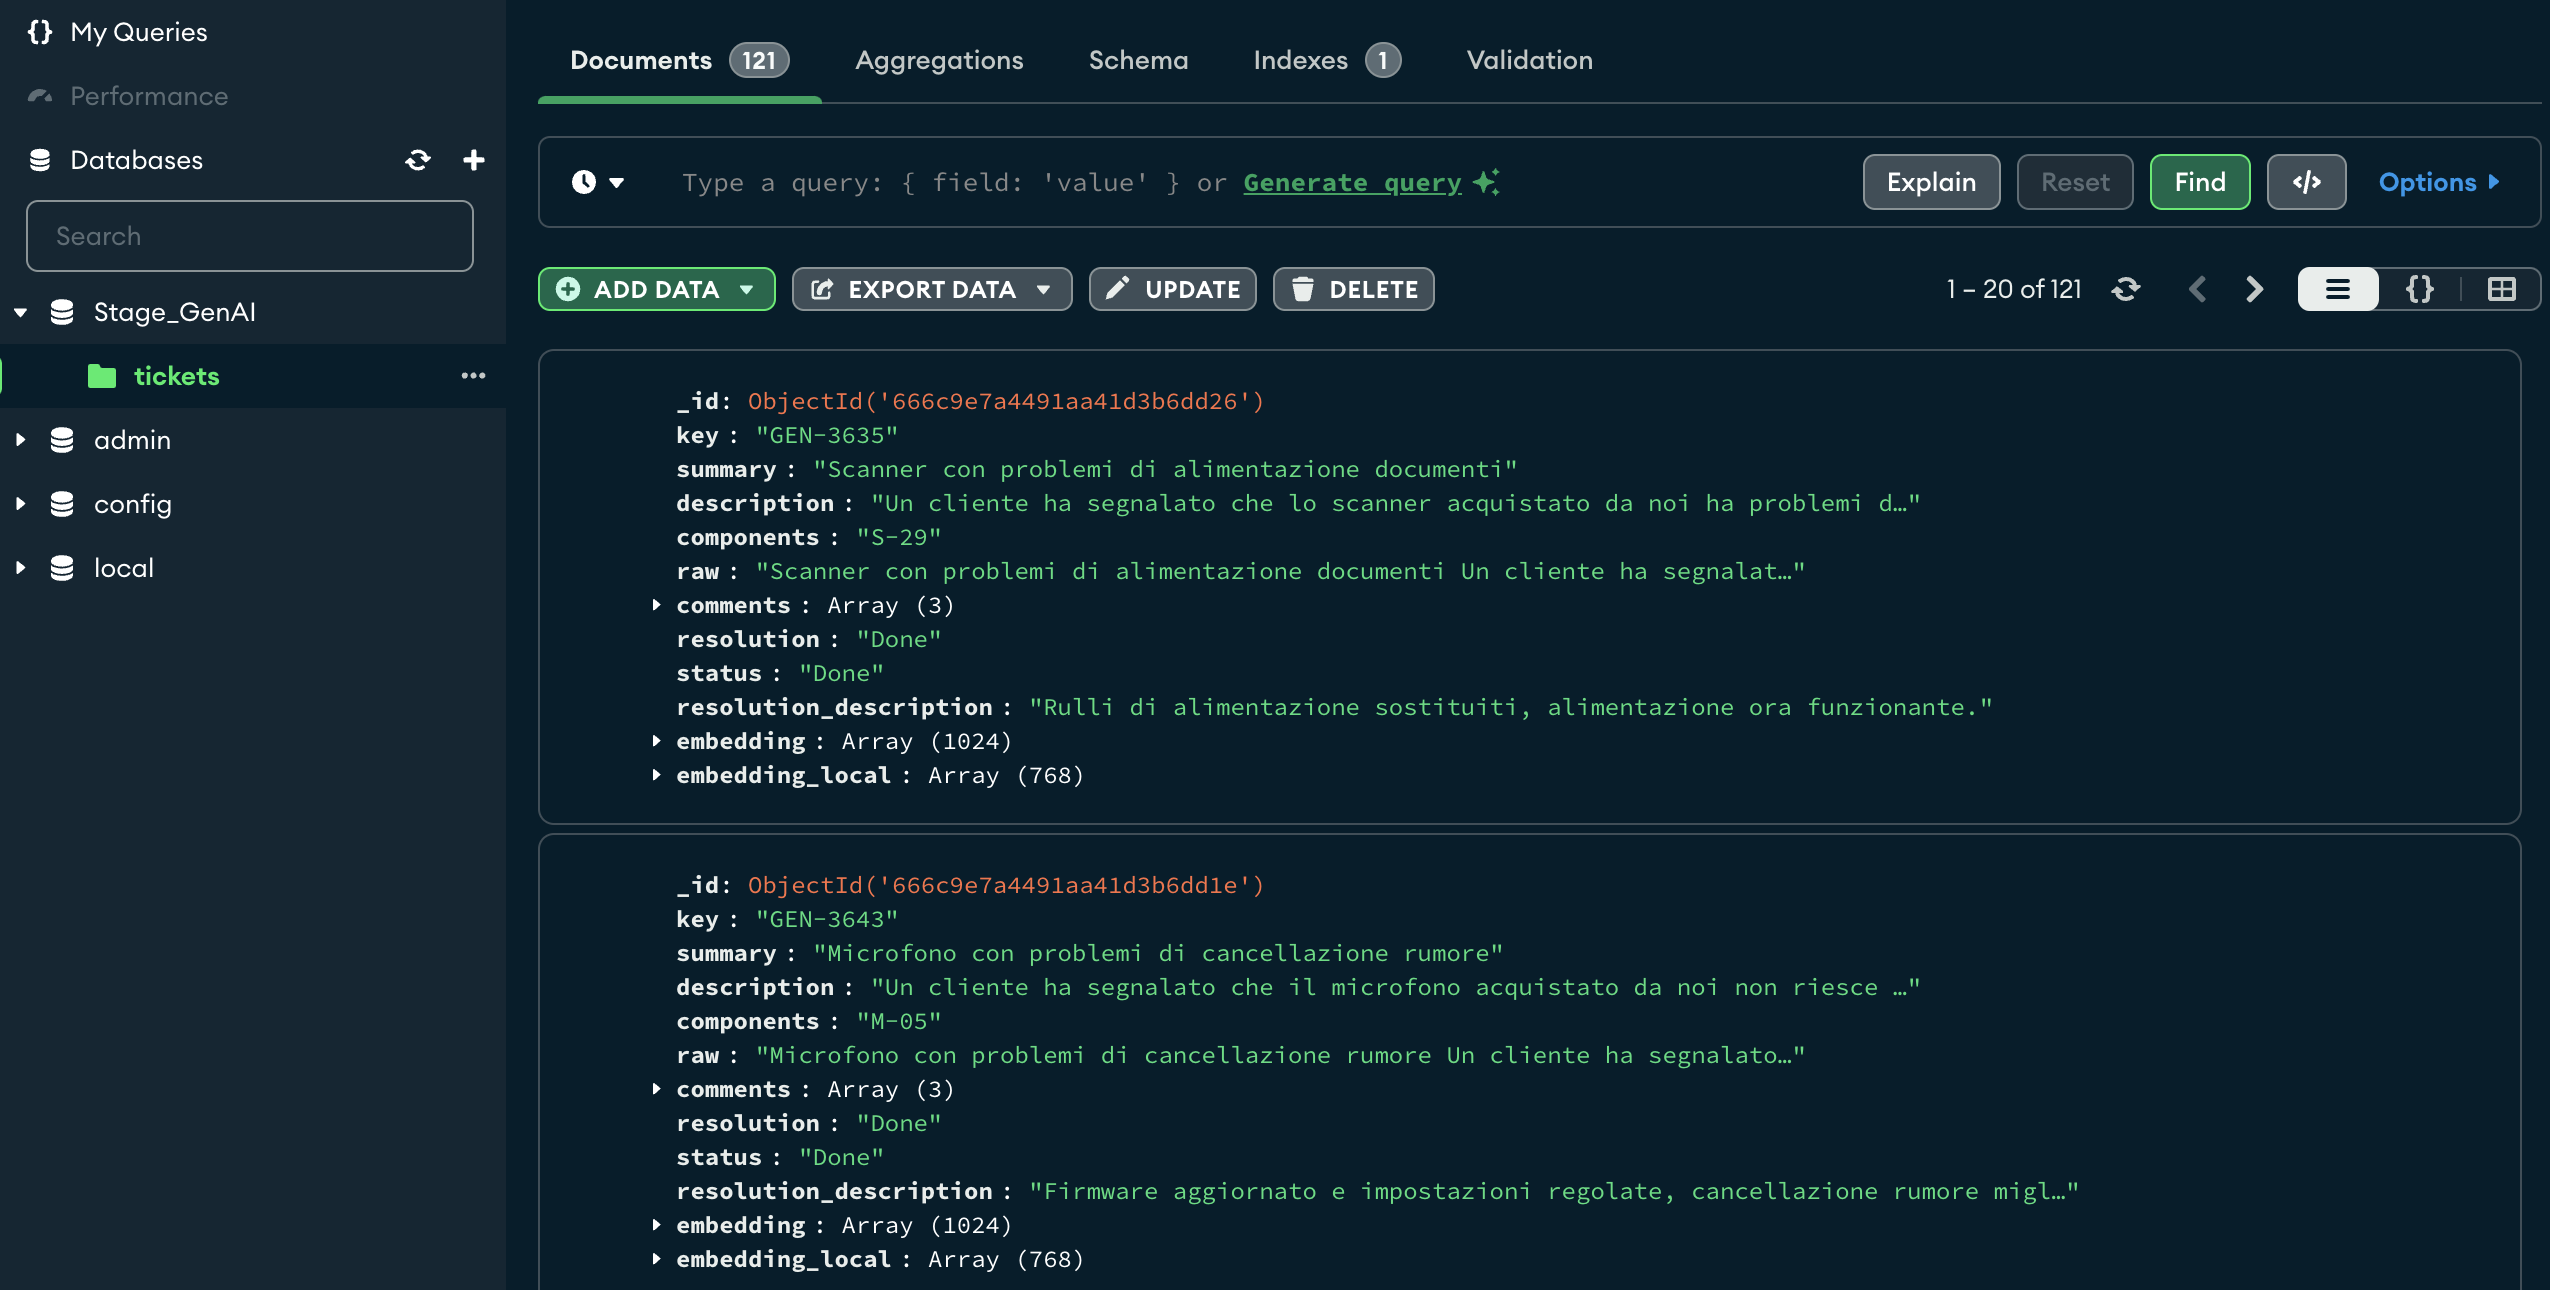
\includegraphics[width=0.65\textwidth]{mongodb.png}
    \caption{Esempio di visualizzazione di documenti su MongoDB Compass}
    \label{fig:MongoDB}
\end{figure} 
%\noindent Esempio di utilizzo di un termine nel glossario \\
%\gls{api}. \\

%\noindent Esempio di citazione in linea \\
%\cite{site:Agile-manifesto}.

%\noindent Esempio di citazione nel pie' di pagina \\
%citazione\footcite{womak:lean-thinking} \\

\section{Tipologia di clientela}
Durante il mio periodo di \textit{stage} , ho avuto modo di osservare la diversità dei clienti che si rivolgono a Zero12 s.r.l. Tra i committenti dei vari progetti sviluppati dall'azienda, ci sono numerose aziende operanti nel medesimo settore, le quali richiedono consulenze sulle tecnologie di cui l'azienda è \textit{partner}.
L'azienda collabora anche con clienti provenienti da settori diversi, come ad esempio il settore della moda, con \textit{brand} di lusso che richiedono lo sviluppo di applicazioni \textit{web} o \textit{mobile} per la gestione dei propri prodotti o servizi.

\section{Propensione all'innovazione}
L'azienda è fortemente orientata all'innovazione e alla sperimentazione di nuove tecnologie, sin dalla sua fondazione.
L'azienda si propone ai suoi nuovi clienti come \textit{Innovation advisor} e grazie a delle sessioni con il cliente, riesce a sviluppare soluzioni innovative in linea con le esigenze del cliente. Essendo \textit{parter} \gls{awsg}, l'azienda è particolarmente incentrata nella ricerca di innovazione in ambito \textit{cloud}.
In aggiunta, i dipedenti stessi organizzano eventi interni in cui vengono discusse nuove tecnologie o assitono alla presentazione di nuove tecnologie, portando cosi nuove idee anche non inerenti all'ambito \textit{cloud}, segno di una forte curiosità e propensione all'innovazione.

%\section{Organizzazione del testo}

%\begin{description}
    %\item[{\hyperref[cap:introduzione]{Il primo capitolo}}] descrive ...
    %\item[{\hyperref[cap:lo-stage]{Il secondo capitolo}}] descrive ...
    
    %\item[{\hyperref[cap:descrizione-stage]{Il terzo capitolo}}] approfondisce ...
    
    %\item[{\hyperref[cap:conclusioni]{Il quarto capitolo}}] approfondisce ...
    
%\end{description}

%Riguardo la stesura del testo, relativamente al documento sono state adottate le seguenti convenzioni tipografiche:
%\begin{itemize}
	%\item gli acronimi, le abbreviazioni e i termini ambigui o di uso non comune menzionati vengono definiti nel glossario, situato alla fine del presente documento;
	%\item per la prima occorrenza dei termini riportati nel glossario viene utilizzata la seguente nomenclatura: \emph{parola}\glsfirstoccur;
	%\item i termini in lingua straniera o facenti parti del gergo tecnico sono evidenziati con il carattere \emph{corsivo}.
%\end{itemize}
